\documentclass{beamer}

\usepackage[ngerman]{babel}
\usepackage{graphicx} % fuer Bilder
\usepackage{listings} % fuer Code
\usepackage{lmodern}

%\usetheme{Goettingen}

%% Formatierung des Sourcecodes
\DeclareFontShape{OT1}{cmtt}{bx}{n}{<5><6><7><8><9><10><10.95><12><14.4><17.28><20.74><24.88>cmttb10}{}
\definecolor{eclipse-violet}{rgb}{0.50, 0.0, 0.46}
\definecolor{eclipse-green}{rgb}{0.25, 0.50, 0.37}
\definecolor{eclipse-blue}{rgb}{0.17, 0.0, 1.00}
\lstset{
 language=C++, % fuer c++ code style
 showstringspaces=false,
 basicstyle=\ttfamily\small,
 keywordstyle=\bfseries\color{eclipse-violet},
 commentstyle=\color{eclipse-green},
 stringstyle=\color{eclipse-blue}
}

\title{Prozesslenkung: Hierarchische Zustandsautomaten II}
\subtitle{Implementierung Hierarchischer Zustandsautomaten}
\author{Katja Kirstein, Anne-Lena Kowalka, Marian Triebe, Eugen Winter}
\date{\today}

\begin{document}

\begin{frame}
 \titlepage
\end{frame}

%% Themen uebersicht
\begin{frame}
 \frametitle{Themen}
 \begin{itemize}
  \item Grundlagen GoF
  \item Externe Statevariablen
  \item Guards/Choice Points
  \item Entry und Exit Code
  \item History
  \item Timer
 \end{itemize}
\end{frame}

%% fsm Systemgrenzen
\begin{frame}
 \frametitle{Systemgrenzen}
 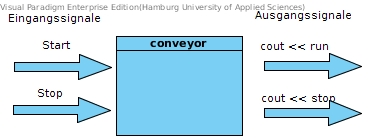
\includegraphics[scale=.7]{img/Systemgrenzen_fsm_gof.jpg}
\end{frame}

%% fsm Automat
\begin{frame}
 \frametitle{Automat}
\end{frame}

%% Switch Case Implementierung
\begin{frame}
 \frametitle{Implementierung I}
\end{frame}

%% Matrix Implementierung
\begin{frame}
 \frametitle{Implementierung II}
\end{frame}


%% GoF fsm Beispiel (Klassendiagramm)
\begin{frame}
 \frametitle{GoF State Pattern Struktur}
 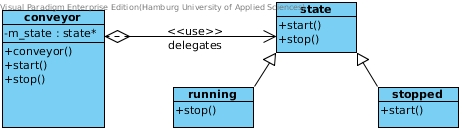
\includegraphics[scale=.6]{img/fsm_gof.jpg}
 \begin{itemize}
  \item Kontext-Klasse (conveyor)
  \item Zustands Basisklasse (state)
  \item Zust\"ande (running, stopped)
 \end{itemize}
\end{frame}

%% Grundlagen GoF
\begin{frame}
 \frametitle{Grundlagen GoF}
 Die klassiche GoF Implementierung hat einige schw\"achen
 \begin{itemize}
  \item Hoher Speicherverbrauch, da jeder Zustand im Speicher gehalten werden muss, auch wenn diese eigentlich nicht verwendet werden
  \item Der h\"ohere Speicherverbrauch kann allerdings mit dem Placement New Operator umgangen werden
  \item Kontext muss eventuell immer mit \"ubergeben werden
 \end{itemize}
\end{frame}


%% GoF fsm States in Code I
\begin{frame}
 \frametitle{GoF States in Code I}
 \begin{itemize}
  \item Alle States erben von einer Oberstate Klasse
  \item Der Oberstate implementiert alle Events aller Zust\"ande als leere virtuelle Funktion
  \item Der jeweilige Zustand implementiert nur seine eigenen Events, nicht relevante
  Events werden an die leeren Methoden der Basisklasse weitergereicht
 \end{itemize}
\end{frame}

%% GoF fsm States in Code (Header)
\begin{frame}[fragile]
 \frametitle{GoF States in Code (Header)}
 \begin{lstlisting}
class state {
 public:
  virtual ~state() { }
  virtual void start() { }
  virtual void stop() { }
};

class running : public state {
 public:
  void stop();
};

class stopped : public state {
 public:
  void start();
};
 \end{lstlisting}
\end{frame}

%% GoF fsm States in Code (Implementierung/CPP)
\begin{frame}[fragile]
 \frametitle{GoF States in Code (Implementierung)}
 \begin{lstlisting}
// transition running -> stopped
void running::stop() {
  new (this) stopped;
  cout << "stop() / stop" << endl;
}

// transition stopped -> running
void stopped::start() {
  new (this) running;
  cout << "start() / run" << endl;
}
 \end{lstlisting}
\end{frame}

%% GoF fsm Kontext Klasse
\begin{frame}
 \frametitle{GoF Kontext Klasse}
 \begin{itemize}
  \item Sicht von au{\ss}en auf die FSM
  \item Dient als Delegator zu den Zust\"anden
  \item Bedient alle Eingangssignale durch Funktionen
 \end{itemize}
\end{frame}

%% GoF fsm Konext Klasse
\begin{frame}[fragile]
 \frametitle{GoF Kontext Klasse in Code}
 Header:
 \begin{lstlisting}
class conveyor {
 public:
  conveyor() : m_state(new stopped) { }
  ~conveyor() { delete m_state; }
  void start();
  void stop();
 private:
  state* m_state;
};
 \end{lstlisting}
 Implementierung:
 \begin{lstlisting}
void conveyor::start() {
  m_state->start();
}

void conveyor::stop() {
  m_state->stop();
}
 \end{lstlisting}
\end{frame}

%% Schritte zum erstellen einer FSM
\begin{frame}
 \frametitle{Schritte zum erstellen einer FSM}
 \begin{enumerate}
  \item Erstellen der Systemgrenzen
  \item Erstellen einer FSM
  \item Umwandlung in Code
  \begin{itemize}
   \item Kontextklasse, Funktionsnamen als Eingangssignale
   \item Basisklasse f\"ur Zust\"ande erstellen
   \item Zustandsklassen erben von der Basisklasse und implementieren nur die eigenen Reaktionen neu
  \end{itemize}
  \item Pr\"ufen ob Code und Systemgrenzen/Diagramm zusammenpassen
  \begin{itemize}
   \item Sind alle Eingangssignale als Funktionen zu finden?
   \item Werden alle Ausgangssignale verwendet/ausgegeben?
   \item Die Namen f\"ur Eingangssignale/Ausgangssignale sollten konsistent sein, da Fehler sonst vorprogrammiert!
  \end{itemize}
 \end{enumerate}
\end{frame}

%% �bung GoF
\begin{frame}
 \frametitle{\"Ubung Lichtschalter}
 Erstellt die Systemgrenzen, Automatendiagramm, und Code eines Lichtschalters (An und Aus Button). (15 Min)
\end{frame}

%% Externe Statevariablen
\begin{frame}
 \frametitle{Externe Statevariablen}
 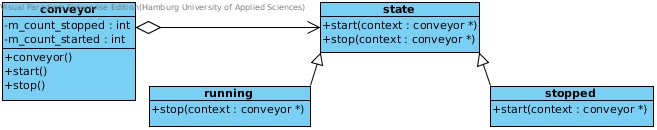
\includegraphics[scale=.44]{img/fsm_externe_state_var.jpg}
\end{frame}

%% Implementierung von externen Statevariablen I
\begin{frame}[fragile]
 \frametitle{Implementierung von externen Statevariablen I}
 \begin{lstlisting}
class conveyor {
  friend class running;
  friend class stopped;
 public:
  conveyor()
      : m_state(new stopped),
        m_count_stopped(0),
        m_count_started(0) { }
  ~conveyor() { delete m_state; }
  void start();
  void stop();
 private:
  state* m_state;
  int m_count_stopped;
  int m_count_started;
};
\end{lstlisting}
\end{frame}

%% Implementierung von externen Statevariablen II
\begin{frame}[fragile]
 \frametitle{Implementierung von externen Statevariablen II}
 Header:
 \begin{lstlisting}
class state {
 public:
  virtual ~state() { }
  virtual void start(conveyor* context) { }
  virtual void stop(conveyor* context) { }
};

class running : public state {
 public:
  void stop(conveyor* context);
};

class stopped : public state {
 public:
  void start(conveyor* context);
};
 \end{lstlisting}
\end{frame}

%% Implementierung von externen Statevariablen III
\begin{frame}[fragile]
 \frametitle{Implementierung von externen Statevariablen III}
 Implementierung:
 \begin{lstlisting}
// transition running -> stopped
void running::stop(conveyor* context) {
  ++context->m_count_stopped;
  new (this) stopped;
}

// transition stopped -> running
void stopped::start(conveyor* context) {
  ++context->m_count_started;
  new (this) running;
}

void conveyor::start() {
  m_state->start(this);
}

void conveyor::stop() {
  m_state->stop(this);
}
 \end{lstlisting}
\end{frame}

%% Guards
\begin{frame}
 \frametitle{Guards}
 Guard Automat:
\end{frame}

%% Guard Implementierung
\begin{frame}[fragile]
 \frametitle{Guards Implementierung}
 Implementierung:
 \begin{lstlisting}
// transition stopped -> running
void stopped::start(conveyor* context) {

  ++context->m_count_started;

  if (context->m_count_started <= 2) {
    new (this) running;
  } else {
    return;
  }
}
 \end{lstlisting}
\end{frame}

%% Choice Points
\begin{frame}
 \frametitle{Choice Points}
\end{frame}

%% �bung Guards
\begin{frame}
 \frametitle{\"Ubung Lichtschalter II}
\end{frame}

%% Entry/Exit Code 1
\begin{frame}
 \frametitle{Entry/Exit Code in HSM }
 \begin{itemize}
  \item Zustandswechsel d\"urfen Hierarchieebenen nicht \"uberspringen
  \item exit() wird durchgef\"uhrt, wenn Signale in der Hierarchie "nach oben" weitergereicht werden
  \item entry() wird  durchgef\"uhrt, wenn Signale in der Hierarchie "nach unten" weitergereicht werden
 \end{itemize}
\end{frame}

%% Entry/Exit Code 2
\begin{frame}
 \frametitle{Entry/Exit Code in HSM }
 \begin{itemize}
  \item Beispiel exit: State S12 erh\"alt Signal e\newline\newline
  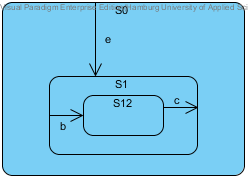
\includegraphics[scale=.6]{img/beispiel_exitSM}
 \end{itemize}
\end{frame}

%% Exit Code 3
\begin{frame}[fragile]
 \frametitle{Entry/Exit Code in HSM }
 \begin{lstlisting}
 //State S12 erhaelt Signal e
 void StateS12::sigE() {
   exit();
   new (this) StateS1;
   sigE();
 }
 \end{lstlisting}
 \begin{itemize}
  \item die exit-Funktion ist in jedem Zustand definiert
  \item wenn auch der Top-Zustand nicht auf ein Signal reagiert, sollte dieser z.B. eine
  failure-Methode haben, um den Fehler anzuzeigen
 \end{itemize}
\end{frame}

%% Entry Code 1
\begin{frame}
 \frametitle{Entry/Exit Code in HSM  }
 \begin{itemize}
  \item Beispiel entry: State S1 erh\"alt Signal b\newline\newline
  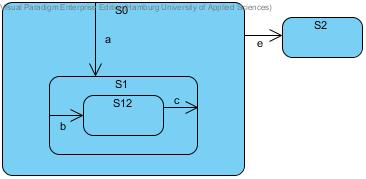
\includegraphics[scale=.6]{img/beispiel_entrySM}
 \end{itemize}
\end{frame}

%% Entry Code 2
\begin{frame}[fragile]
 \frametitle{Entry/Exit Code in HSM }
 \begin{lstlisting}
//State S1 erhaelt Signal b
void StateS1::init(T* t) {

  //t ist ein Pointer auf die Kontextklasse
  void* history = t->getStateFromHistory(StateS1ID);

  if(history != 0) {
    memcpy(this, &history, 4);
  } else {
    new (this) StateS12;
    entry();
  }
  init();
}
 \end{lstlisting}
\end{frame}

%% Entry Code 3
\begin{frame}[fragile]
 \begin{itemize}
  \item die entry-Funktion ist in jedem Zustand definiert
  \item init() f\"uhrt dazu, dass -sofern ein Substate bereits in der History vorliegt- dieser direkt betreten wird; ansonsten wird er neu erzeugt
  \item der erneute init()-Aufruf darf in der vorletzten bzw. letzten Hierarchie-Ebene nicht stattfinden (ansonsten Endlosschleife) ????????? korrekt??
 \end{itemize}
\end{frame}

%% History 1
\begin{frame}
 \frametitle{History}
 \begin{itemize}
  \item Implementierung der flachen History
  \item die history-Funktion  wird in der exit-Funktion aufgerufen
  \item die Kontextklasse h\"alt ein History- Array,
  in dem sich die Subzust\"ande mittels history-Aufruf eintragen (Index-Zuordnung z.B. \"uber enums)
 \end{itemize}
\end{frame}

%% History 2
\begin{frame}[fragile]
 \frametitle{History}
 \begin{itemize}
  \item Beispiel: S1 tr\"agt sich in History-Tabelle ein
 \end{itemize}
 \begin{lstlisting}
  //StateS1 history-Funktion
  voidS StateS1::history(T* t) {

    //t ist ein Pointer auf die Kontextklasse
    t->setHistory(State::StateID::StateS1_ID,
                  this);
  }
 \end{lstlisting}
 \begin{itemize}
  \item der Parameter StateS1ID gibt den Index in der History-Tabelle in der Kontextklasse an
 \end{itemize}
\end{frame}

%% History 3
\begin{frame}[fragile]
 \frametitle{History}
 \begin{itemize}
  \item setHistory in der Kontextklasse:
 \end{itemize}
 \begin{lstlisting}
  void setHistory(int ID, State* ptr) {
    history_[ID] = *((void**) ptr);
  }
 \end{lstlisting}
 \begin{itemize}
  \item ptr wird zun\"achst auf void** gecastet, damit man mit einer weiteren Dereferenzierung * an die virtuelle Funktionstabelle des Zustands gelangt
 \end{itemize}
\end{frame}

%% History 4
\begin{frame}[fragile]
 \frametitle{History}
 \begin{itemize}
  \item getStateFromHistory in der Kontextklasse:
 \end{itemize}
 \begin{lstlisting}
  void* getStateFromHistory(int ID) {
    return history_[ID];
  }
 \end{lstlisting}
 \begin{itemize}
  \item \"uber seine ID kann der Zustand sich seine History -sofern eine vorliegt- aus der History-Tabelle in der Kontextklasse holen
 \end{itemize}
\end{frame}

%% Timer 1
\begin{frame}[fragile]
 \frametitle{Timer}
 \begin{itemize}
  \item Definition der Zeit-Messung eines Timers:\newline\newline
  $\bullet$ \textbf{Absolut}: L\"ose aus \textbf{am} 24.12.2014\newline
  (Zeit vergangen seit 01.01.1970 00:00)\newline\newline
  $\bullet$ \textbf{Relativ}: L\"ose aus \textbf{in} 10 Sekunden\newline
  (Zeit vergangen seit Start des Timers)
 \end{itemize}
\end{frame}

%% Timer 2
\begin{frame}[fragile]
 \frametitle{Timer}
 \begin{itemize}
  \item Definition des Zeit-Intervalls eines Timers:\newline\newline
  $\bullet$ \textbf{Periodisch}: L\"ose alle 100 Millisekunden aus\newline\newline
  $\bullet$ \textbf{One-Shot}: L\"ose einmalig in 10 Sekunden aus
 \end{itemize}
\end{frame}

%% Timer 3
\begin{frame}[fragile]
 \frametitle{Timer}
 \begin{itemize}
  \item Ereignis beim Ausl\"osen eines Timers:\newline\newline
  $\bullet$ \textbf{Pulse Message}: Sende eine Pulse Message\newline\newline
  $\bullet$ \textbf{Signal senden}: Sende ein Signal (z.B. SIGTERM)\newline\newline
  $\bullet$ \textbf{Thread starten}: Starte einen bestimmten Thread
 \end{itemize}
\end{frame}

%% Timer 4
\begin{frame}[fragile]
 \frametitle{Timer}
 \begin{itemize}
  \item Erforderliche Schritte f\"ur die Nutzung eines Timers:\newline\newline
  \textbf{1.} Timer Objekt erstellen\newline\newline
  \textbf{2.} Entscheiden, wie man benachrichtigt werden m\"ochte (Pulse Message, Signal, Thread) und dementsprechend das \textbf{struct sigevent} initialisieren\newline\newline
  \textbf{3.} Entscheiden, welche Art von Timer man w\"ahlt (relativ vs. absolut \& one-shot vs. periodisch)\newline\newline
  \textbf{4.} Timer starten
 \end{itemize}
\end{frame}

%% Timer 5
\begin{frame}[fragile]
 \frametitle{Timer}
 Beispiel f\"ur die Erstellung eines Timers (1/2):
 \begin{lstlisting}
// 1.
timer_t timerid;
struct sigevent event;
struct itimerspec timer;

// 2.
SIGEV_PULSE_INIT(
  &event, // struct sigevent
  coid,   // Connection ID of message receiver
  SIGEV_PULSE_PRIO_INHERIT, // Priority
  MY_CODE_TIMER, // Code for pulse handler
  MY_VALUE_TIMER // Value for pulse handler
);
 \end{lstlisting}
\end{frame}

%% Timer 6
\begin{frame}[fragile]
 \frametitle{Timer}
 Beispiel f\"ur die Erstellung eines Timers (2/2):
 \begin{lstlisting}
// 3. Create timer with realtime clock
timer_create(CLOCK_REALTIME, &event, &timerid);

// Setup the timer (2s delay, 1s reload)
// it_value = one-shot value
// it_interval = reload value
timer.it_value.tv_sec = 2;
timer.it_value.tv_nsec = 0;
timer.it_interval.tv_sec = 1;
timer.it_interval.tv_nsec = 0;

// 4. Start the timer
timer_settime(timerid, 0, &timer, NULL);
 \end{lstlisting}
\end{frame}

%% Timer 7
\begin{frame}[fragile]
 \frametitle{Timer}
 \begin{itemize}
  \item Hinweis f\"ur die Abfrage des Benachrichtigung-Typs:\newline
  \begin{lstlisting}
// Don't read the struct sigevent directly
if(event.sigev_notify == SIGEV_PULSE)

// Use this macro instead
if(SIGEV_GET_TYPE(&event) == SIGEV_PULSE)
  \end{lstlisting}
 \end{itemize}
\end{frame}

%% Timer 8
\begin{frame}[fragile]
 \frametitle{Timer}
 \begin{itemize}
  \item TODO:\newline\newline
  $\bullet$ \textbf{BEISPIEL}: Server, der auf Timer / Clients wartet\newline\newline
  $\bullet$ \textbf{BEISPIEL}: switch-case Refactoring nach Fowler\newline\newline
  $\bullet$ \textbf{BEISPIEL}: Orthogonale Automaten\newline\newline
  $\bullet$ \textbf{BEISPIEL}: F\"unf Pr\"ufungsfragen
 \end{itemize}
\end{frame}

%% Prüfungsfragen
\begin{frame}
 \frametitle{Pr\"ufungsfragen}
 \begin{itemize}
  \item Welche Arten von Implementierungen gibt es?
  \item Wie gehz man Schrittweise vor einen Automaten zu implementieren?
  \item Was ist zu beachten von Statevariablen und die Nachteile die dadurch entstehen?
  \item Wie geht man vor einen Timer zu implementieren?
 \end{itemize}
\end{frame}

\end{document}
